
\chapter{绪论}
\label{chap:introduction}


\section{引言}

从定义上来说,等离子体是由带电粒子和原子构成的具有集体行为的准电
中性物质,被称为除气态,液态和固态之外的物质第四状态。整个宇宙中,等离子体的存在更具普遍性, $99\%$ 以上的物质都处于等离子体状态 \cite{chen1984plasma}
,地球属于剩余的 $1\%$ 。等离子体是由 W. 克鲁克斯在 1879 年发现的,在 1928 年美国科学家
欧文·朗缪尔(Irving Langmuir)和汤克斯(Tonks)首次将“等离子体”
(plasma)一词引入物理学,用来描述气体放电管里的物质形态,并由此开创了一
个崭新的物理学领域。当功率密度大
于 $10^{14}W / {cm}^2$ 时, 绝大多数物质将被电离,形成等离子体。 激光等离子体加速(laser plasma acceleration―LPA) 是1979年由Tajima和Dawson提
出\cite{tajima1979laser}。 LPA利用等
离子体作为加速媒介,等离子体中加速电场强度可达到$E_0 = c{m_e} {\omega}_p /e$,
或者写为$E_0 (V/m) =96 \sqrt{n_0 (cm^{-3} )}$,
其中$n_0$ 是等离子体的电子密度, ${\omega}_p = (4\pi n_0 e^2 /{m_e} )^{1/2}$ 为等离子体波的频率。 所以
当$n_0 = 10 ^{18} {cm} ^{- 3}$ 时,LPA的加速梯度可以达到$96 GV/m$,超过传统射频加速器
三个量级以上。这种新型加速器拥有广阔的前景,然而限于当时激光技术,一直未能在实验上取得突破。 20 世纪 80 年代末期 G. Mourou 等提出
啁啾脉冲放大 (CPA) 技术 \cite{strickland1985compression} ,为实验的发展奠定了基础。近年来,强激光与等离子体作用的研究在实验和理论上得到
迅速发展。

\begin{figure}[!htbp]
  \centering
  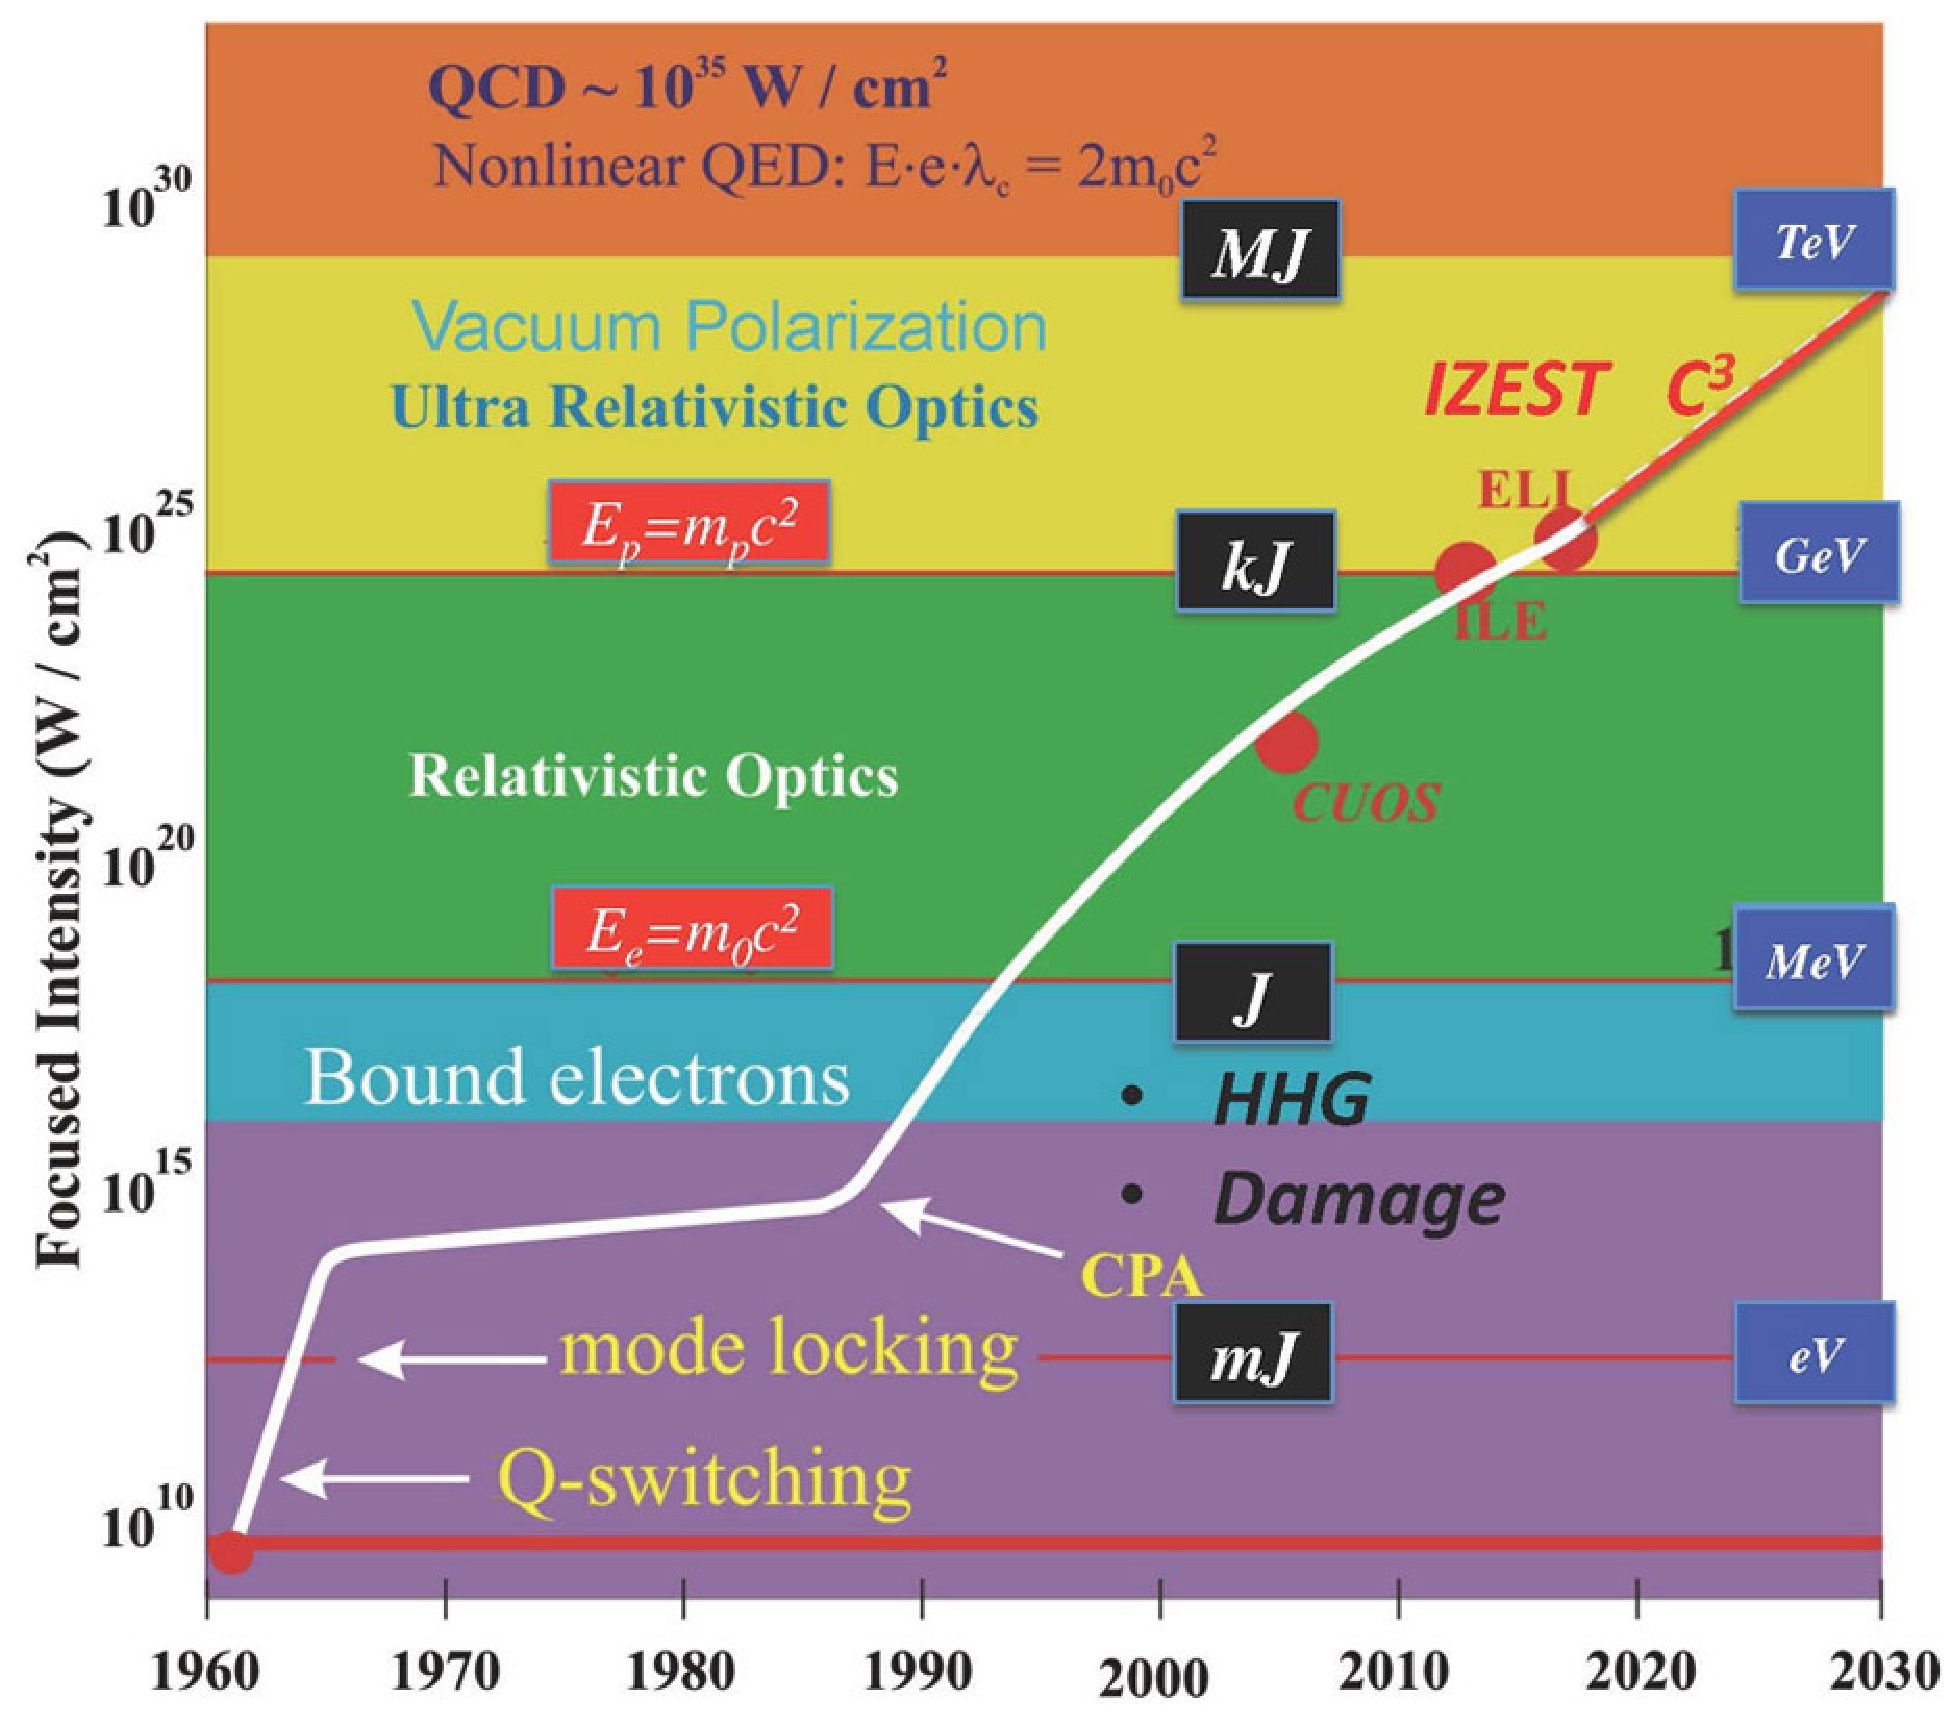
\includegraphics[width=0.4\textwidth]{Img/moraulaser.eps}
  \caption{各种光强对应的物理}
  \label{fig:moraulaser}
\end{figure}


\section{等离子体的描述}

等离子体实际上是由大量带电粒子组成的电离气体,其动力学行为受到长程电磁
力的支配,且其运动规律呈现集体运动特性。由于多自由度以及相互关联性,合理的等离子体描述方法成为理论研究的基础问题。
等离子体物理中常用的基本描述方法有以下三种:单粒子理论,流体
理论,动力学理论。其中动力学理论中常见的有符拉索夫方程和福克 — 普朗克方程以
及粒子模拟方法。




\subsection{单粒子轨道描述方法}
当等离子体碰撞的平均自由程远大于等离子体空间尺度时,粒子间
的碰撞以及带电粒子的自洽场可以忽略,
分析电磁场对带电粒子的作用足以描述其运动。在假设合理的前提下,粒子的轨道描述能够简化问题,并对问题给出定性解释。轨道描述作为讨论粒子间相互作用对等离子体行为影响时的零级近似,是理论上的出发点。经典的平面波与初始静止电子的作用可有;;;模型得到;;;, 其主要结论,地那子在纵向上以二倍激光频率运动,横向上以激光频率震荡,如图(\ref{fig:singleelectron})。
\begin{figure}[!htbp]
  \centering
  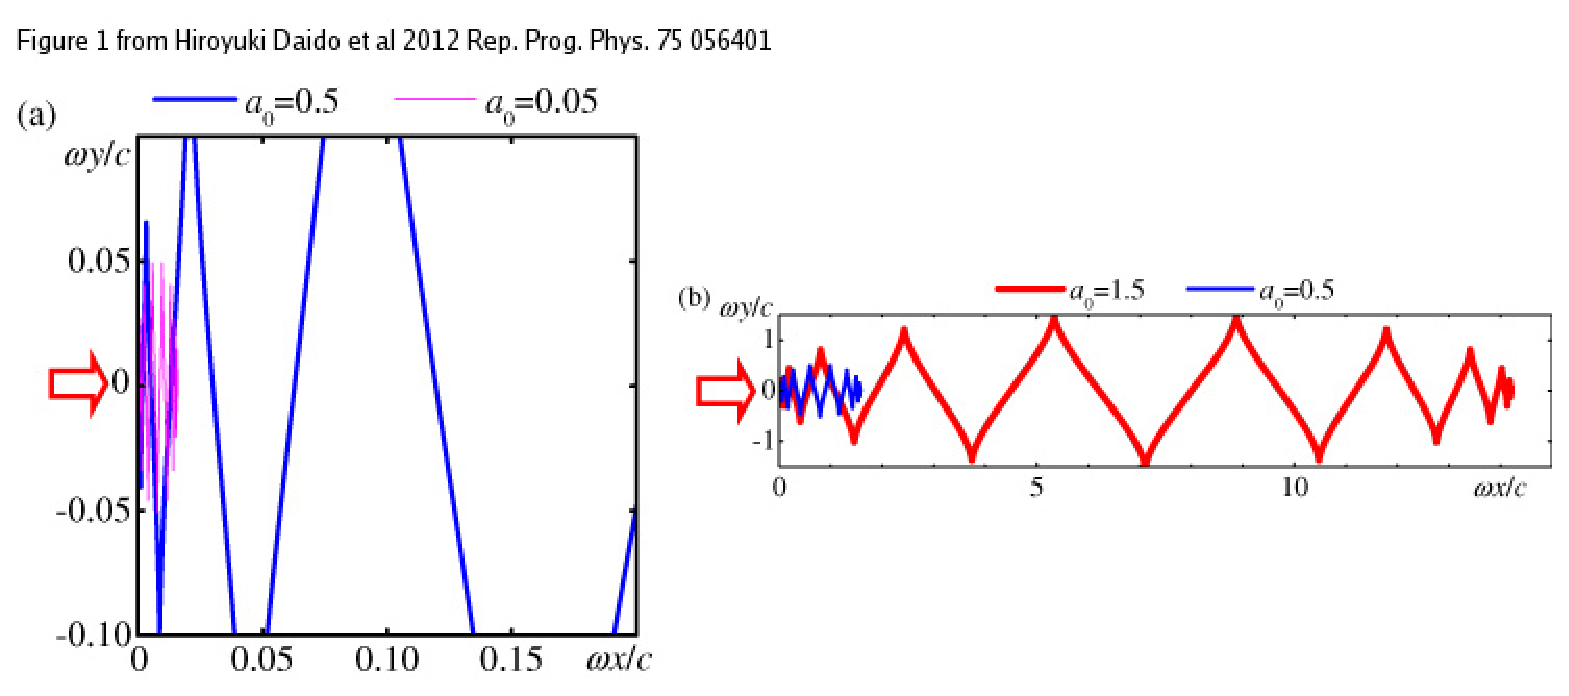
\includegraphics[width=\MyFactor\textwidth]{Img/singElectron2012Trajectory.eps}
  \caption{电子在平面波中的运动}
  \label{fig:singleelectron}
\end{figure}


\subsection{Vlasov模拟和Fokker-Planck模拟方法}
Vlasov模拟和Fokker-Planck模拟是以粒子分布函数为基础,求解分布函数的演化方程,最后根据分布函数和宏观量之间的关系来研究等离子体性质。根据
碰撞相互作用的重要性,可以把动力学方程模拟分成Vlasov模拟和Fokker-
Planck模拟。
当碰撞效应可以忽略时,采用Vlasov模拟,其中a粒子的分布函数满足:

\begin{equation}
\label{eqn:vlasov_distribution}
\partial{f^a}/\partial{t}+\bf{v} \cdot {\nabla}f^a +  \dfrac{q_a }  
{m_a} 
(\bf{E}+ 
\dfrac{1}{v}  \bf{v} \times \bf{B}) \cdot  {\nabla}_v f^a = 0 
\end{equation}     

当碰撞效应不可以忽略时,采用Foker-Planck模拟,其中a粒子的分布函数满足:

\begin{equation}
\label{eqn:foker_distribution}
\partial{f^a}/\partial{t}+\bf{v} \cdot {\nabla}f^a +  \dfrac{q_a }  
{m_a} 
(\bf{E}+ 
\dfrac{1}{v}  \bf{v} \times \bf{B}) \cdot  {\nabla}_v f^a = 
(\partial{f^a}/\partial{t})_{collision}
\end{equation}     


\subsection{流体力学模拟方法}
对于高密度等离子体,由于达到局部热动平衡的弛豫时间很短(皮秒量级),
等离子体状态可作局域热平衡近似,激光等离子体相互作用就可用多温流体
力学描述,并给出电子、离子的输运系数及辐射信息。
\subsection{粒子模拟方法}
粒子模拟方法是通过追踪大量的在自洽
和外加电磁场作用下的带电粒子的运动来研究等离子体集体运动性质的动力学
模拟方法。实际中等离
子体粒子数远超出计算机的计算能力,例如典型
的实验室等离子体(聚变装置中的等离子体)中总粒子数大约是$10^{19} /m^3$ 。很难实现全部粒子跟踪模拟,因此“宏粒子”的概念就非常必要。在等离子体分布函数的
相空间中的一点(x,v)的周围,每个带电粒子对电磁场的贡献和电磁场对粒子
的作用力都基本相同,故周围这些大量带电粒子的运动规律基本相同。
基于此特征,Buneman\cite{buneman1959dissipation}和Dawson\cite{dawson1962one}提出“宏粒子”。忽略宏粒子内部的作用,考虑宏粒子之间,以及宏粒子与场的作用。但是由于点粒子间的库仑碰撞作用,静电噪声太大。随后,Birdsall
和Langdon提出了有限大小粒子模型,将粒子电荷分布等效为云分布。粒子云之
间可以穿越和重叠,当粒子云分离时,遵循库仑力相互作用,重叠时遵循线
性力,解决了粒子间库仑碰撞的问题。宏粒子与粒子云模型,在控制计算误差的同时降低了计算规模,是粒子模拟方法中有效的模型。粒子模拟方法的基本过程如下:(1)粒子的位置,速度,电荷密度和电流密度分布初始化;(2)数值求解Maxwell 方程组(FDTD有限时域差分)更新电磁场分布;(3)由动力学方法更新粒子的位置和速度分布,并由此得到电荷密度和电流密度分布。而后,循环(2),(3)得到等离子体内部粒子和场的信息。
\begin{figure}[!htbp]
  \centering
  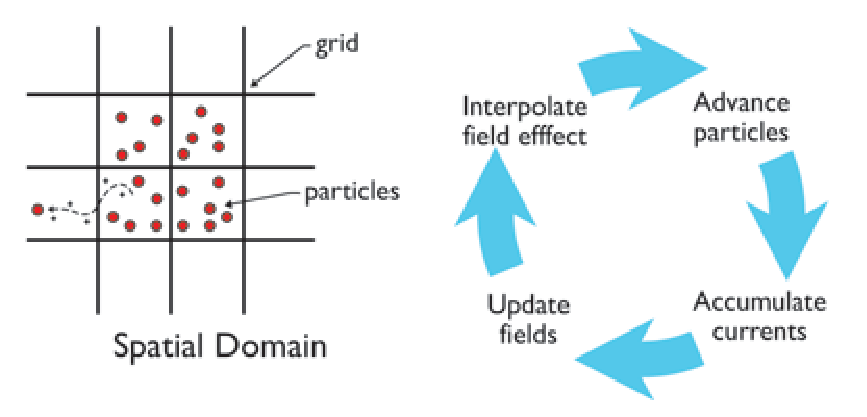
\includegraphics[width=\MyFactor\textwidth]{Img/PIC.eps}
  \caption{PICmodel}
  \label{fig:picmodel}
\end{figure}





\section{激光在等离子体中吸收}




当平面波激光脉冲作用于自由电子时,在一个周期内电子平均动量不变,能量增益为零。然而当激光在等离子体中传播时,集体效应显得更为重要。激光在等离子体中激发等离子体波,其频率为
\begin{equation}
\label{eqn:plasmafrequency}
\omega_p=\sqrt{\frac{e^2 n_e}{\epsilon_0 m \gamma}}
\end{equation}
激光电磁场在等离子体中的色散关系\cite{kruer1988physics}:
\begin{equation}
\label{eqn:chromatic}
{{\omega}_L}^2={{\omega}_p}^2 + c^2 k^2
\end{equation}
因此激光在等离子体中的折射率:
\begin{equation}
\label{eqn:defrection}
\eta=\sqrt{1- \frac{{{\omega}_p}^2}{{{\omega}_L}^2}}
\end{equation}
可以看出当$\omega_p > \omega_L$时, 折射率为实数,激光可以在等离子体中传播,相速度和群速度为:
\begin{equation}
\label{eqn:velocity}
v_{ph}=c/{\eta}, v_g=c \eta
\end{equation}
当$\omega_p = \omega_L$定义了等离子体的临界密度,对于非相对论激光,
\begin{equation}
\label{eqn:criticalDensity}
n_{cr}=\frac{\epsilon_0 m_e {{\omega}_L}^2}{e^2} \approx 1.1 \times 
10^{21} (\frac{\lambda_L}{\mu m})^{-2} {cm}^{-3}
\end{equation}

由于相对论效应的存在,$a>1$时,临界密度值与光强有关,此时临界密度为:
\begin{equation}
\label{eqn:RelcriticalDensity}
n_{cr}=\gamma n_{cr}
\end{equation}
相对论激光的穿透能力相应的提高,而这种非线性现象称为激光的相对论自透明\cite{willingale2009characterization},此时等离子体的折射率为:
\begin{equation}
\label{eqn:Realdefrection}
\eta=\sqrt{1- \frac{n_e}{\gamma n_{cr}}}
\end{equation}
折射率由等离子体密度与激光光强有关。考虑高斯脉冲在均匀密度等离子体中的传播,其折射率受到光强分布的影响,呈类高斯的分布,对于激光光束具有棱镜汇聚的效应,被称作相对论自聚焦\cite{sprangle1987relativistic,sun1987self,chen1993necessary,esarey1997self}。此外等离子体中电子被激光脉冲排开,形成类似通道结构\cite{82},改变等离子体中电子的密度分布,促进激光有质动力自聚焦。同时由于群速度受到光强影响,导致非线性激光自相位调制\cite{83,84},改变激光脉冲的纵向分布。

然而当$\omega_p < \omega_L$时, 
折射率为虚数,激光可以在等离子体中迅速衰减,其作用距离在趋肤深度以内:
\begin{equation}
\label{eqn:skindepth}
l_s=\frac{c}{\omega_p}
\end{equation}


在激光的传播过程中,其能量通过多种作用部分地被等离子体吸收。从碰撞作用的角度讲,激光在等离子
体中的吸收机制分为正常吸收和异常吸收两种。正常吸收也可称为逆轫致吸
收,由粒子之间的碰撞引起,在短波长,小角度入射的情况下主导。异常吸收是指激光能量通过非碰撞机制部分地
转化为等离子体其他形式的波的能量。异常吸收可以分为共振吸收、真空加热、
JxB加热等。下面作简单介绍:
\subsection{逆轫致吸收}
逆轫致吸收主要是由于粒子间的碰撞引起的。在激光场中,电子在横向电场
的作用下进行高频振动, 碰撞效应使得电子的动能转化至等离子体,激光的能量由此被等离子体吸收。
若忽略集体效应和量子效应,当 $ {\hslash} \omega \ll  k_B T_e$ 时,激光线性吸收系数 $K_{ib}$为
\begin{equation}
\label{eqn: laserLinearAbsorbtion}
K_{ib} \approx \frac{Z {n_e}^2}{{T_e}^{3/2} (1-{n_e}/{n_{cr}})^{1/2}}
\end{equation}

其中Z为原子序数, $n_e$ 为电子密度, $n_{cr}$ 为等离子体临界密度, $T_e$ 为电子温度。但
随着激光强度增加,等离子体的温度上升其直接导致电子与离子间的碰撞频率降
低,逆轫致吸收的作用减弱,非碰撞
吸收机制开始增强。部分电子由逆轫致吸收产生
温度低于keV的热电子, 另一部分是由其他吸收机制产生的超热电
子。

\subsection{共振吸收}
共振吸最早由Forslimd\cite{forslund1977theory}和Estabrook\cite{estabrook1978properties}报道。其能量吸收,通过共振方式发生在临界密度面上,是超短超强激
光与物质作用中存在的重要吸收机制。当P偏振的激光以 $\theta$角斜入射到非均匀密度等离子体中,在临界密
度面 $n=n_{cr} cos(\theta)$ 发生反射,此时激光电场在临界密度面附近沿密度梯
度方向的分量,驱动电子在等离子体密度梯度方向来回振荡,激发电
子等离子体波,最后通过各种阻尼机制如朗道阻尼、波破等将能量转化为电子能量。
共振吸收基本上是一种线性吸收,在给定的临界密度面附近等离子体密度标
长 $L=(1/n \times  dy/dx )^{-1}$ 的情况下,等离子体的密度振荡和静电波的振幅都
与激光电场成正比。共振吸收系数与密度标长和激光入射角有关系\cite{kruer1988physics},在密
度标长不变的情况下,最大吸收对应的角度满足
\begin{equation}
\label{eqn: resonaceformula}
sin(\theta)=0.8 (\omega L/c)^{-1/3}
\end{equation}
其中 $\omega$为激光频率。
超热电子的温度与激光强度之间有经验上的
定标率\cite{forslund1977theory}
\begin{equation}
\label{eqn: resonacescale}
T_{hot} \approx 14(I{\lambda}^2)^{1/3} {T_b}^{1/3}
\end{equation}
其中 I 是以 $10^{16} W/{cm}^2$ 为单位的激光光强, $\lambda$是以$\mu m$为单位的激光波长, $T_b$ 是以
$keV$为单位的背景电子温度。
\subsection{真空加热}
真空加热\cite{bulanov1994interaction, 
gibbon1992collisionless}又称为“Not-so-resonant, resonant absorption”,由
Brunel于1987年首次提出\cite{brunel1987not}。真空加热与共振吸收共同存在于激光与物质作用表面,作用强度受密度分布影响。密度标长较大时,共振吸收主导,激光电场能够在临界密度面附近驱动强等离子体波,并将能量传递至电子。密度标长较小(小于一个激光波长),共振条件无法满足,此时激光通过非共振地耦合到
静电等离子体波中,此时真空加热主导。如果电子的振荡幅度大于等离子体密度标长,等离子体中的电子
被拉到真空中;当电场相位反转,电子又被拉回等离子体中形成超热电子,或与
离子场作用辐射出x射线光子。
做简单的估计,考虑平面电磁场波以$\theta$ 角入射到密度梯度十分“陡峭”的等
离子体上,在电磁波的反射面上产生 $E=2 E_0 sin{\theta}$ 的驱动电场。根据泊松方程,
单位面积上被拉到真空中的电子数目为
$\frac{2 E_0 sin{\theta}}{4 \pi e}$
,根据电子所吸收的能量,真空
加热造成的能量损失率与电子的最大振荡速度($v_{osc}=eE_0/m \omega$)和入射角 $\theta$的关系
为
\begin{equation}
\label{eqn: vocummHeating}
f_{vh} \propto v_{osc} sin^3 \theta
\end{equation}
因此真空加热与激光强度成线性正比关系,而且增大入射角也可增加能量的吸收。


\subsection{JxB加热}

JxB加热是1985年由Kruer 和Estabrook提出的\cite{kruer1985j},它是由激光的有质动力
的振荡部分产生。在等离子与真空的交界面上,由于趋肤效应,激光的电场和磁场
将在趋肤深度的范围内进入到高密等离子体中,因此JxB加热机制依赖于真空等
离子体界面附近的激光光强的梯度。考虑在真空等离子体交界面附近的电子流体元,其运动
方程可写为\cite{wilks1997absorption}
\begin{equation}
\label{eqn: movingEquation}
\partial{\bf{p}}/\partial{t}+ \bf{v} \cdot 
\nabla{\bf{p}}=-e[\bf{E}+\frac{\bf{v} \times \bf{B}}{c}]
\end{equation}

其中 $\bf{p}=\gamma m_0 \bf{v}$
$\gamma=\frac{1}{\sqrt(1-\frac{v^2}{c^2})}=\frac{1}{\sqrt(1-\frac{{\bar{p}}^2}{{\gamma}^2})}$
${\bar{p}}^2 = {p_{osc}}^2/{m_e}^2c^2$
在圆偏振光下 $\gamma = \sqrt{1+{\bar{p}}^2}$ 
,线偏振光下$\gamma = \sqrt{1+{\bar{p}}^2/2}$ 。利用 $\bar{p}$ 和矢势 $\bf{A}$ ,
重写(\ref{eqn: movingEquation}),可以获得电子流体元的动量的纵向分量
\begin{equation}
\label{eqn: movingEquationX}
\partial{\bf{p}_L}/\partial{t}=e \nabla \phi -m_0 c^2 
\nabla{(\gamma -1)}
\end{equation}
式中第一项是静电力引起的,第二项是相对论有质动力项。由此,有质动力势可
得
\begin{equation}
\label{eqn: ponderomotivePotential}
U_p=m_0 c^2 (\gamma -1)
\end{equation}



取非相对论近似,则(\ref{eqn: ponderomotivePotential})式就是有质动力势的标准表达形式。
如果在激光与等离子体相互作用的过程中,电子受到这个势场的作用,电子
的能量从势场中获得,那么热电子的温度定标律为\cite{malka1996experimental}

\begin{equation}
\label{eqn: ponderomotiveScale}
T_{hot}=(\sqrt{1+\frac{I {\lambda}^2}{2.8 \times 10^{18}}}-1) \cdot 511 
keV
\end{equation}

Malka和Miquel\cite{malka1996experimental}使用脉宽在300-500fs,
波长为$1.056\mu m$的激光垂直入射到固体靶,靶面激光功率密度为 $2 \times 10^{19}W/{cm}^2$。
在靶后$0^\circ$和$22^\circ$的位置,测量热电子温度,发现在$0^\circ$方向电子温度
满足(\ref{eqn: ponderomotiveScale})式,而在其他方向热电子温度与 $I^{\alpha}$ 成比例,例如在$22^\circ$方向,
$\alpha \approx 0.28$。
考虑非相对论形式的JxB加热,电子受到的
力由下式给出:
\begin{equation}
\label{eqn: ponderomotiveForce}
f_p=-{\frac{\partial}{\partial{x}}}{\frac{m v^2_{osc}}{2} 
frac{4{\omega}^2_0}{{\omega}^2_{pe}} e^{-2{\omega}_{pe} 
X/c[\frac{1+cos2\omega t}{2}]} }
\end{equation}


位于等离子体内深x处的电子受到的力。电子加热源于有质动力中两倍于激光频率时间振荡项。激光与等离子体作用面上电子处于这种振荡状态,
其中一部分电子所处的位相使得它们通过非绝热的碰
撞从振荡中获得能量,进入密度更高的等离子体。获得能量的电子数量由振荡力的大小所决定。对于相对论强度激光与物质作用, J x B加热电子的效率十分显著,甚至超过其他集中加热机制成为主导作用。对于非相对论激光,当驱动电场远大于JxB驱动
项时,真空加热的作用大于JxB加热。如下情形\cite{malka1996experimental}: $2E_Lsin\theta > V_{osc} B_L$ 或 $sin{\theta}> 
(v_{osc} / c)({\omega}_0/{\omega}_{pe})$







\section{激光电子加速}

在激光等离子体电子加速提出之前,1956 年Fainberg 就提出了利用电子束激发等离子体尾波场的方
案,相应的粒子加速称为等离子体尾波场加速\cite{esarey1996overview} 。1990 年Nakajima采用相同
的方法利用能量为500MeV、脉宽10ps 、电量为10nC 的多电子束激发密度为
$( 2-8 )\times 10^{12} {cm}^3$ ,长度为1m 长的等离子体,获得的电子最大能量增益为
30MeV\cite{nakajima1990plasma}。
最早提出利用激光在等离子体中形成电子等离子波并加速电子的方案的是
Tajima 等人,他们在在1979 年分析利用纵向的激光尾波场作为电子加速场的可
能性,并依照当时的激光技术,提出了利用激光拍频波激发激光尾波场的方案\cite{tajima1979laser}。对应于不同的激光技术条件,人们提出了多种激光尾波场
加速的方案:激光拍频波加速(PBWA)\cite{tajima1979laser, tang1985dynamics} 、脉冲链尾波场加速
(RLPA)\cite{umstadter1994nonlinear}、激光尾波场加速(LWFA)\cite{malka2002electron,geddes2004high,mangles2004monoenergetic,faure2004laser},自调制激光尾波场加速
(SM-LWFA)\cite{sprangle1992propagation,modena1995electron}。

当激光脉冲在小于临界密度的等离子体中传播时,在光脉冲的纵向有质动
力作用下等离子体中的电子向前运动,离子由于惯性大保持位置。激光电场随传播而消失,而正负电荷分离而产生的静电势使得电子在平衡位置附近作纵向振荡,形成电子等离子体波。该等离子波是由激光脉冲激发且存在于激光脉冲之后,被称为激光尾波。它的相速度与激光脉冲在等离子体中传播的群速度相同,激光尾波场以同样的相速度向
前传播。激光尾波场的强度受尾波场本身波破极限的限制,其幅度可以比通常的射频场加速器高三个量级。当等离子体
的密度达到 $n_0=10^{18} {cm}^3$ 时,尾波场的强度可以达到 $E =100 GV / m$ 。电子在尾波
场中的正向加速区域得到加速,反之则减速。

在2002 年,利用激光
尾波场加速,获得200MeV的电子\cite{malka2002electron},但其单能性较差。2004年,美国的Geddes\cite{geddes2004high}利用预等离子体通道导引一束相对论强度的超短
激光脉冲,增加了激光的有效传播距离,结果产生了能量$80MeV \pm 1.8MeV$ ,发散角$3mrad$ 的准单能电子束。此后不久Mangles等人\cite{mangles2004monoenergetic},通过改变等离子体
密度,发现在适当的情形下,可以产生能散度小于$6\%$ 的中心能量为70MeV 的单
能电子束。法国的Faure等人\cite{faure2004laser},利用更高强度的激光脉冲,实现了激
光脉宽与尾波长度相当的条件下的空泡加速,得到了能量为170MeV
的准单能电子束。2006年,激光尾波场加速电子在能量和稳定性上又取得了进一
步的突破。Leemans等人利用毛细管对激光进行引导,获得了1GeV的准单能电子
束\cite{leemans2006gev}。Faure
等人\cite{faure2006controlled}将两束激光同轴反向传输,一束为低强度的注入脉冲,另一束作为主脉冲。
利用主脉冲激光产生强的尾波场,而在两光束重叠区,形成驻波场,在驻波
场有质动力的作用下,部分初速合适的电子被尾波场捕获并加速。实验结果,能量保持在$117 \pm 7MeV$,能散度$11
\pm 2\%$,发散角$5.8 \pm 2mrad$,重复率高。
2009年,帝国理工大学的Kneip等人利用$200TW$激光脉冲($55fs$,$a  \approx 3.9$)自引导通过密度为 $5.7 \times10^{18} cm^{-3}$ 长度为10 mm等离子体,得到准单能的800 MeV电子束 \cite{kneip2009near}。 2010年UCLA的Clayton等人将110TW激光脉冲(60
fs,$a \approx 3.8$)聚焦到1.3 cm的气体腔中($1.5 \times 10^{18} cm^{-3}$)
,利用电离注入机制将加
速电子的最高能量再次提高到1.45 GeV连续谱能量 \cite{clayton2010self}。



\subsection{激光离子加速}

离子由于惯性较大,在典型光强下,无法在激光场中直接加速。实验中,离子加速源于电子离子间静电分离势其束具有流准直性良好(发射度在$mm \cdot mrad$)量级,粒子数目多($10^{10}-{10}^{13} 
$),ps量级脉冲宽度等特点。因此激光离子加速得到的粒子束可应用于,质子照相 \cite{borghesi2002macroscopic,romagnani2005dynamics}、离子束
癌症治疗\cite{malka2004practicability,bulanov2002feasibility}、快点火\cite{roth2001fast} 以及常规加速器中的
粒子注入源\cite{haseroth1996physical}等。







最早的离子加速可以追溯到1963 年, W. I. Linlor 等从在实验中
通过长脉冲激光 (0.2 J , 40 ns , $5 \times {10}^9 W/{cm}^2$ ) 与等离子体作用,得到约 1keV
的离子束\cite{linlor1963ion}。1997 
年,T. Ditmire  利用 150 fs , $2 \times {10}^{16} W/{cm}^2$ 的激光脉冲与 Xe
原子团簇作用,产生MeV 的 Xe 离子,比小分子相互作用产生的离子
能量高 4 个量级\cite{ditmire1997high} 。 2000 年 E. L. Clark 通过50 J , 
~1 ps , $5 \times {10}^{19} W/{cm}^2$
的 Vulcan 激光脉冲与 125$\mu m$ Al 靶相互作用,产生 18MeV 的加速质子\cite{clark2000measurements} 。


同年, R. A. Snavely使用NOVA (~48 J , ~500fs , $3 \times {10}^{20} W/{cm}^2$)
激光作用在固体靶上观察到截止能量为 58 MeV 的质子\cite{snavely2000intense}。
2009 年, S.Gaillard 使用Trident 
激光(~80 J , ~700fs , $1.5 \times {10}^{20} W/{cm}^2$)于微结构铜靶作用,获得最高能量67.5 MeV 的质子\cite{gaillard2011increased}。

离子加速能量不断提高的同时,降低能散以获得准单能的离子束是激光离
子加速的另一个重要研究课题。2002年Esirkepov等人通过三维数值模拟提出了用双层
靶实现准单能离子加速的构想\cite{esirkepov2002proposed}
,并在随后得到了实验的证实。2006年Schwoerer等人利用双层靶获得了中心能量为1.2MeV,能散度为$25\%$的
准单能质子束 \cite{schwoerer2006laser}。Hegelich
等人也利用这种复合靶得到了能散在$17\%$,能量在3MeV每核子的准单能离子
束 \cite{hegelich2006laser}。



现有的激光离子加速实验,由于其激光光强以及靶厚度的原因,大部分归于靶后鞘层加速(TNSA)\cite{hatchett2000electron}。


\subsection{鞘层加速机制}
靶后鞘层加速机制(Target Normal Sheath Acceleration)是目前最广泛认可的
一种加速机制,简称TNSA\cite{hatchett2000electron}。其简化物理图像:电子在靶前被激光加热,传播至靶后并形成德拜长度量级的鞘层场。鞘层场对靶后表面的离子进行加速。这个物理过程可以用等离子体的真空自由膨胀模型 \cite{mora2003plasma,mora2005thin}来描述,

\begin{figure}[!htbp]
  \centering
  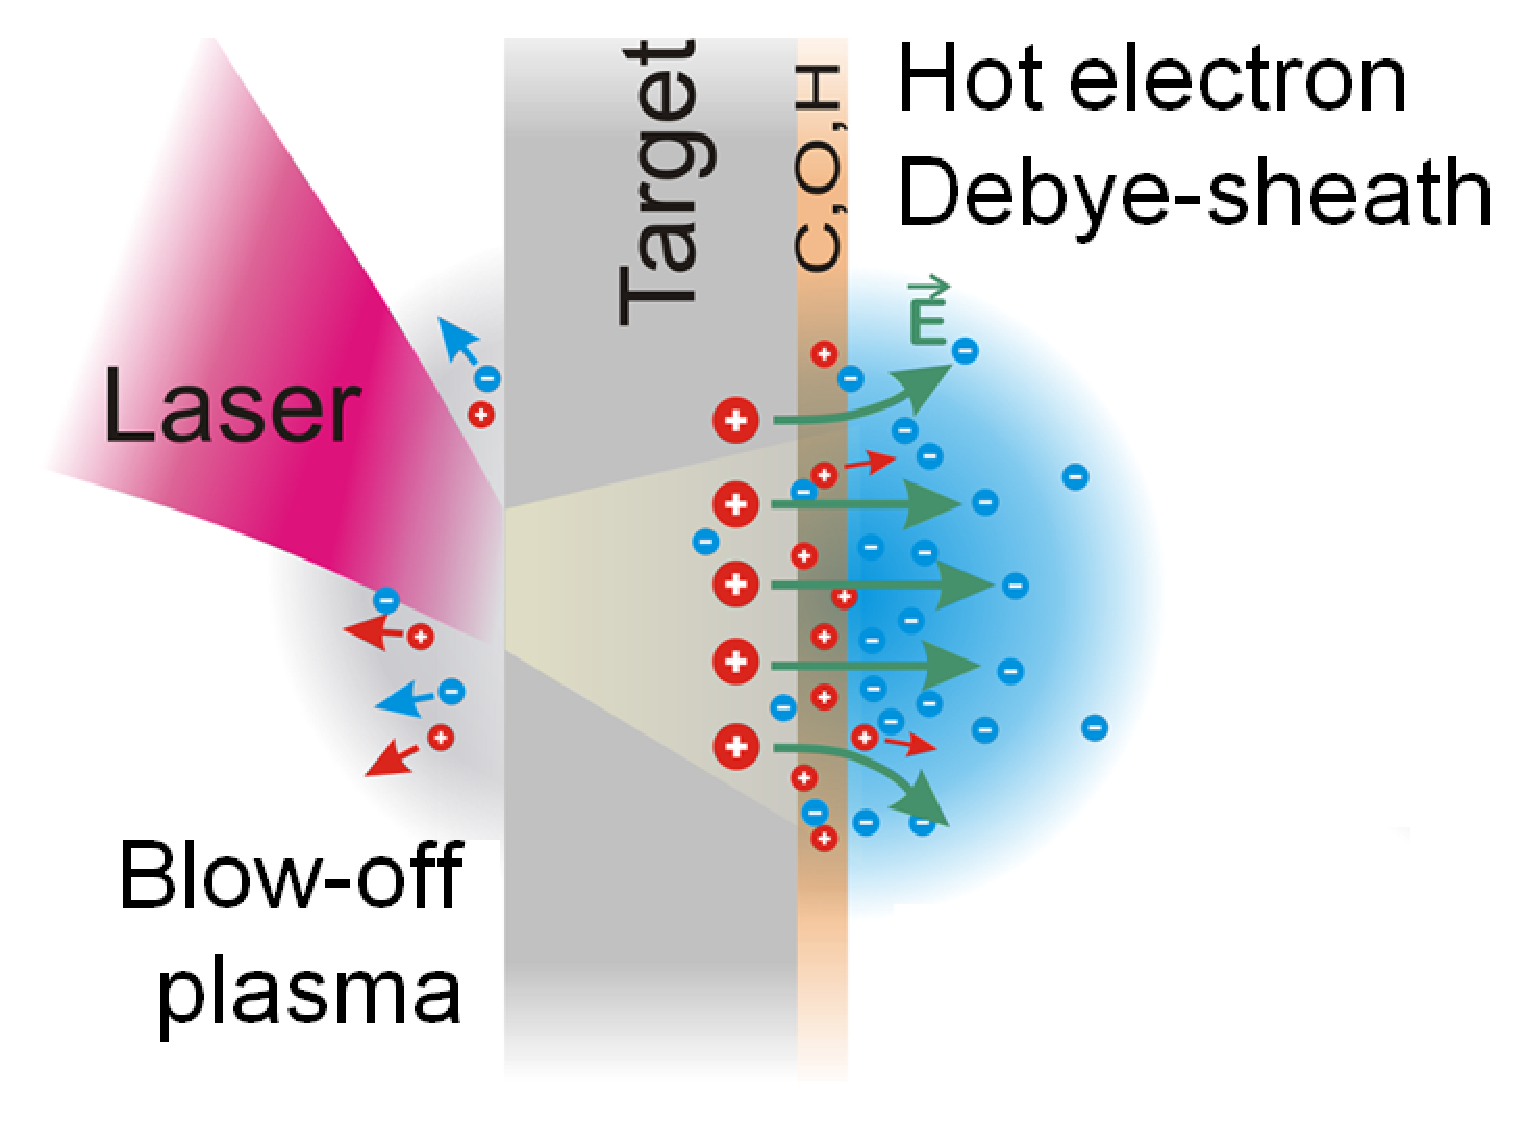
\includegraphics[width=\MyFactor\textwidth]{Img/TNSA.eps}
  \caption{TNSA示意图}
  \label{fig:TNSA}
\end{figure}


 模型初始条件为:假设离子
静止均匀分布于原点左侧, 电子全空间分布, 其分布服从玻尔
兹曼(Boltzmann)统计:
\begin{equation}
\label{eqn:electronBoltz}
n_e = n_{e0} exp(\frac{e\phi}{T_e})
\end{equation}
电子静电势满足泊松方程:

\begin{equation}
\label{eqn:electronBoltz}
\frac{d^2\phi}{dx^2} =4\pi (n_e-Z_i  n_i) 
\end{equation}

这里$n_e$ , $T_e$ 表示靶后的热电子的密度和温度,$n_i$ , $Z_i$ 为离子的密度和电量。靶
后鞘层电场的特征长度为电子的德拜长度:
\begin{equation}
\label{eqn:debyeLength}
\lambda_D = (T_e /4πn_e e^2)^(1/2)
\end{equation}

初始时刻电场的最大值为:
\begin{equation}
\label{eqn:maxField}
E_{sheath,0}=\sqrt{\frac{2}{e_N} \frac{T_e}{e {\lambda}_D}}=(\frac{8 
\pi}{e_N} 
n_e T_e)^{1/2}
\end{equation}

这里$e_n \approx 2.71828$为欧拉常数。此后等离子体的自由膨胀可以通过求解连续性
方程和运动方程得到自相似解,其离子的速度前沿为:
\begin{equation}
\label{eqn:frontVelocity}
v_f=2c_s ln(\tau + \sqrt{1+{\tau}^2})
\end{equation}
其 中$\tau = \omega_{pi} t / \sqrt{2e_N}$,  $\omega_{pi} = (4\pi Z_i n_{e0} 
e^2/m_i )^{1/2}$ 为 离 子 等 离 子 体 频 率,$c_s =
(Z_i k_B T_e /m_i )^{1/2}$ 为离子声速。相应的离子加速的最大能量为:
\begin{equation}
\label{eqn:maxEnergy}
\epsilon_i = 2 Z_i T_e{ln \left [ \frac{\omega_{pi} 
t}{\sqrt{2e_N}}+\sqrt{(\frac{\omega_{pi}t}{\sqrt{2e_N}})^2+1} \right ]}^2
\end{equation}
通过这种自相似解得到的电荷分离。 以上的讨论适用于厚靶,对于靶的厚度为d的等离子
体,在$\tau_L \ll t_e=2d/c $时,电子等温膨胀模型有效。当$\tau_L \approx t_e$ 时,或者 $\tau_L \gg t_e$ 的情况,则不适用。











\subsection {激波加速机制}
以上介绍靶后的离子群的鞘层场加速机制,这一
源于靶前的离子群的加速机制。
对于一个垂直于固体靶入射的激光,其纵向的有质动力不停的推动电子往
前跑,激光就像钻孔一样不停的朝靶内推进,这个加速过程也叫做打洞加速
机制(hole boring acceleration)。激光的打洞速度由激光的光压和离子动量平衡决
定:
\begin{equation}
\label{eqn:holeboringEqualibrium}
n_i m_i v_s^2 = (1 + R)I_L /c
\end{equation}
固体靶离子加速机制
其中R为激光的反射率,相应的形成的离子静电激波的速度为:
\begin{equation}
\label{eqn:shockVelocity}
v_s=\sqrt{\frac{(1+R)I_L}{n_i m_i c^3}c}= a_L\sqrt{\frac{(1+R)m_e n_c}{2m_i n_i}}
\end{equation}
激波前的静止离子被激波反弹,得到速度$v_i = 2v_s$ 。激波的马赫数被定义为:
\begin{equation}
\label{machDefine}
M = v_s /c_s
\end{equation}
这里$c_s =\sqrt{Zk_B T_e/ m_i}$ 为离子声速。Silva [101]等人的理论和PIC模拟研究表明
高强度的激光脉冲和固体靶相互作用过程中可以产生高马赫数(2-3)的静电激
波。被激波反弹的离子达到固体靶后的时候,其能够进一步被鞘层场加速到更
高的能量 [101, 102]。当靶足够薄:
\begin{equation}
\label{eqn:thickLimit}
l < 4 \lambda_D M^2/Z_i
\end{equation}
此时到达靶后的离子的最大速度大于鞘层场此时加速离子的最大速度,激波加
速机制能够超越鞘层加速机制而占据主导地位。


\subsection{光压加速机制}

经过几十年的发展,TNSA机制已被证实,但是很难通过优化靶结构明显进一步提高离子束流品质。理论研究表明对应于的给定激光强度,存在最佳的靶厚使得
激光的光压和等离子体的静电分离势
平衡\cite{esirkepov2006laser,yan2008generating,macchi2009light},此时加速离子能量最高。

\begin{equation}
\label{eqn:separation_potential}
a_0 \propto \theta = \frac{n_e l}{n_c {\lambda}_0}
\end{equation}     


这里$\theta$为靶的面密度,为归一化的靶密度和厚度的乘积。满足条件时,激光
穿透靶,由于光压作用将波前部分靶整体推出,其过程可由光帆模型描述。光帆模型中,靶中电子层比作帆,而离子比作船,激光在薄膜靶前表面被反射,光压作用于电子,从而带动靶整体运动,实现离子的加速。与TNSA相比,激光到离子的能量转化效率有数量级上的提高,能量和能散得到显著的提高。这
种加速机制叫做光压加速机制。激光能量通过多普勒频移效应转化为靶中粒子能量,而主要是离子能量(因为离子和电子速度相同,而质量高出三个数量级)。


\begin{equation}
\label{eqn:doplor}
\omega_r = \omega_0/ 4{\gamma}^2
\end{equation}
这里$\omega$为靶运动的相对论因子。随着靶速度的增加,反射光子能量降低,激光与离子间能量转化效率提高。
2004年T. Esirkepov等人\cite{esirkepov2004highly}用线偏振激光在$10^{23} W/cm^2$ 的激光强度下在
三维模拟中看到了这种离子光压加速的现象,他们把这个机制叫做活塞加速机
制,意思是激光像一个活塞一样把整个靶都推出来,从而得到准单能的GeV量
级的离子束。 对于以速度v运动的靶,激光的光压为:

\begin{equation}
\label{eqn:piston}
P_{rad}=R\frac{c-v}{c+v} \frac{2I_0}{c}
\end{equation}这里R是在靶的坐标系下激光的反射率。靶的运动方程为:
\begin{equation}
\label{eqn:targetMove}
\frac{d}{dt}(\beta \gamma) =\frac{2I(t-z/c)}{\rho lc} R \frac{1-\beta}{1+\beta}
\end{equation}
这里$\beta=v/c$,$\gamma=1 \sqrt{1-{\beta}^2}$ , $\rho$,$l$为靶的质量密度和厚度。靶加速的最终速
度$\beta_f$取决于激光的能量密度$F=\int{I dt}$。对于激光反射率$R = 1$,有:
\begin{equation}
\label{eqn:reflectionIndex}
\beta_f=\frac{(1+\epsilon)^2-1}{(1+\epsilon)^2-1}, \epsilon=\frac{2F}{\rho l c^2} =2\pi \frac{Zm_e a^2_0 \tau}{A m_p \pi \sigma}
\end{equation}
其中$\sigma= \frac{n_0l}{nc \lambda}$为靶的面密度,
$\tau$为激光脉冲长度。相应的可以得到离子加速的最大
能量:
\begin{equation}
\label{eqn:ionMaxenergy}
\epsilon_i \approx m_i c^2(\frac{3a_0^2 \tau}{8 \pi n_0 l m_i 
c})^{1/3}=m_i c^2(\mu s \tau/T)^{1/3}
\end{equation}
这里, $\mu=\frac{m_e Z}{m_i}$, $s=\frac{a^2}{\theta}$。


以上考虑的是靶速度接近相对论光速,其反射率$R=1$的情形。而对于非相
对论速度运动的靶($\beta \ll 1$)。离子的能量可以估计为:
\begin{equation}
\label{eqn:ionMaxenergyapprox}
\epsilon_i \approx \approx 2 m_i c^2(\mu R s \frac{\tau}{T})^{2}
\end{equation}

光压加速机制有效地提高了,激光到离子的能量转化效率高,出射离子束流单能性好,方向性等。然所需条件较高, 超过$10^{23} W/cm^2$激光强度 ,以及$100 nm$以下的靶厚度,以及很好的对比度($10^{-10}$以下)。
理论研究表明,对于圆偏振激光,其有质动力不含$2\omega$的振荡项,因此震荡项引起的电子各向同性加热得到抑制,光压更稳定地推动电子层且间接推动离子,因此降低了光压加速机制需要的激光强度\cite{yan2008generating,qiao2009stable,robinson2008radiation,klimo2008monoenergetic}。在这一过程中,离子激光传播方向的相图随着时间呈现内螺旋的稳定结构,由于和常规射频加速器中的稳相加速过程非常类似,被称为稳相加速机制\cite{yan2008generating}。目前较好的实验结果,2009年Henig\cite{henig2009radiation}在实验上得到了准单能$20-40MeV C^{6+}$离子,验证了稳相加速机制。

\begin{figure}[!htbp]
  \centering
  \begin{subfigure}[b]{\MySubFactor\textwidth}
    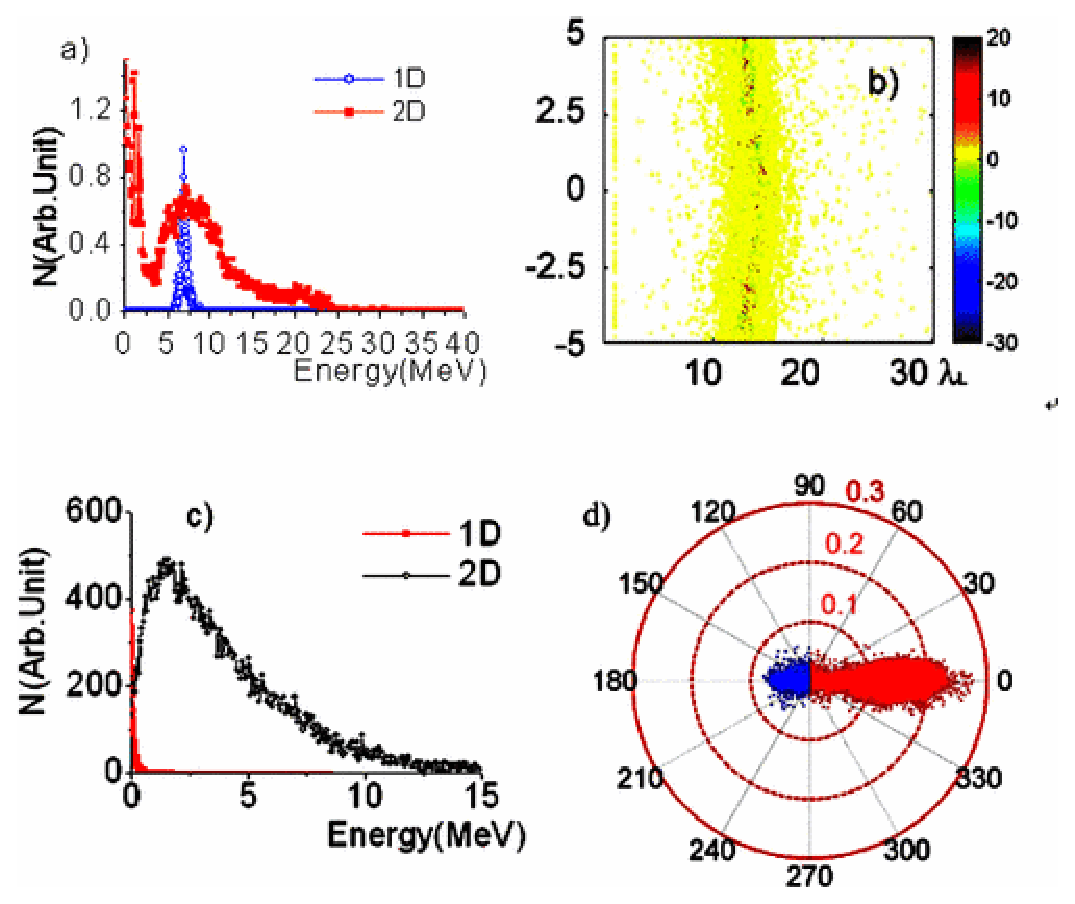
\includegraphics[width=\textwidth]{Img/PSA1.eps}
    \caption{}
    \label{fig:psa1}
  \end{subfigure}%
  ~%add desired spacing
  \begin{subfigure}[b]{\MySubFactor\textwidth}
    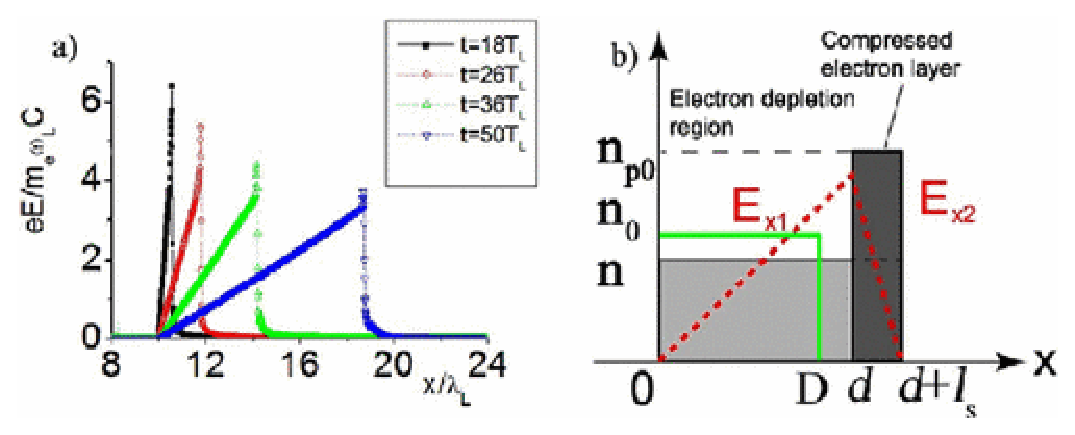
\includegraphics[width=\textwidth]{Img/PSA2.eps}
    \caption{}
    \label{fig:psa2}
  \end{subfigure}
  \caption{稳相加速机制(a)理论研究,(b)实验结果}
  \label{fig:psa}
\end{figure}






\section{论文安排}
